%%%%%%%%%%%%%%%%%%%%%%%%%%%%%%%%%%%%%%%%%
% University/School Laboratory Report
% LaTeX Template
% Version 3.1 (25/3/14)
%
% This template has been downloaded from:
% http://www.LaTeXTemplates.com
%
% Original author:
% Linux and Unix Users Group at Virginia Tech Wiki 
% (https://vtluug.org/wiki/Example_LaTeX_chem_lab_report)
%
% License:
% CC BY-NC-SA 3.0 (http://creativecommons.org/licenses/by-nc-sa/3.0/)
%
%%%%%%%%%%%%%%%%%%%%%%%%%%%%%%%%%%%%%%%%%

%----------------------------------------------------------------------------------------
%	PACKAGES AND DOCUMENT CONFIGURATIONS
%----------------------------------------------------------------------------------------

\documentclass{article}

\usepackage[version=3]{mhchem} % Package for chemical equation typesetting
\usepackage{siunitx} % Provides the \SI{}{} and \si{} command for typesetting SI units
\usepackage{graphicx} % Required for the inclusion of images
\usepackage{natbib} % Required to change bibliography style to APA
\usepackage{amsmath} % Required for some math elements 
\usepackage[utf8]{inputenc}

\setlength\parindent{0pt} % Removes all indentation from paragraphs

\renewcommand{\labelenumi}{\alph{enumi}.} % Make numbering in the enumerate environment by letter rather than number (e.g. section 6)

%\usepackage{times} % Uncomment to use the Times New Roman font

%----------------------------------------------------------------------------------------
%	DOCUMENT INFORMATION
%----------------------------------------------------------------------------------------

\title{Image to text} % Title

\author{Suraj Kiran\\Nakul A\\Umesh U\\Shinoj} % Author name

\date{\today} % Date for the report

\begin{document}

\maketitle % Insert the title, author and date



% If you wish to include an abstract, uncomment the lines below
% \begin{abstract}
% Abstract text
% \end{abstract}

%----------------------------------------------------------------------------------------
%	SECTION 1
%----------------------------------------------------------------------------------------

\section{Abstract}

Character recognition is one of the most
interesting areas of pattern recognition and artificial
intelligence. Image to character recognition extracts
the relevant information and automatically enters it
into electronic database instead of the conventional
way of manually retyping the text. it is a vast field with a number of varied
applications such as social networking, legal industry,
banking, health care industry etc. Image to text conversion can be used to catagorize,analyse big data without any human correction or human
effort, Automatic number plate recognition and
Handwritten Recognition. It contributes
immensely to the advancement of an automation
process and can improve the interface between man
and machine in numerous applications. Several
research works have been focusing on new
techniques and methods that would reduce the
processing time while providing higher recognition
accuracy. Now it is possible to scan documents as an
image and to make it editable and searchable for
further information processing.

%----------------------------------------------------------------------------------------
%	SECTION 2
%----------------------------------------------------------------------------------------

\section{Introduction}
Aim is to create an Android application which can recognize text from image taken using camera and convert it to a human editable form \textit{ex word,pdf etc}.\\
Artificial intelligence and image recognition are the key principle behind working of this application.

\subsection{Edge Detection}
A set of connected pixels that forms a boundary between two
disjoint regions is known as an edge. The task of segmenting
an image into regions of discontinuity is done using edge
detection. Edges usually occur on the boundary of two
different boundaries in an image. Edge detection helps to
clearly identify the changes in region of an image where gray
scale and texture change in the regions of an image. There
are many available edge detection techniques for extracting
edges from images such as Robert, Prewitt and Sobel which
were not much efficient. Then in 1986 John. F. Canny
developed an algorithm which provided high probability of
edge detection and error rate.
\subsection{Canny Algorithm}
This algorithm focuses mainly on three main aims of low
error rate, minimize distance between real edge and detected
edge and minimum response i.e. one detector response per
edge to detect the edges in an image.
\subsection{ Image Segmentation}
Image segmentation is another important aspect necessarily
required to divide an image into regions or categories which
then helps to identify correctly the object in an image.
Segmentation functions on the properties shown by the pixels
in an image, every pixel which belongs to same category has
similar gray scale value whereas pixels of different categories
have dissimilar values. Segmentation is often one of the
critical steps in analyzing the images because additional
overhead of moving to each new pixel of an image while
working with object in an image. Once image segmentation is
done successfully, the other stages in image analysis are
much easier. While considering a fully automatic conversion
algorithm, the success of image segmentation is partial and
sometimes requires manual intervention. Segmentation
mainly has two main objectives: 1) divide or decompose the
image into parts for further processing, 2) perform change in
organizing the pixels of image into higher-level units so that
the objects become more meaningful.



%----------------------------------------------------------------------------------------
%	SECTION 3
%----------------------------------------------------------------------------------------
\newpage
\section{Related works}

\subsection{Image Parsing to Text Description}
\textbf{\small \\Benjamin Z. Yao, Xiong Yang, \\Liang Lin, Mun Wai Lee and Song-Chun Zhu}
\\\\\\
Fast growth of public photo and video sharing websites,
such as “Flickr” and “YouTube”, provides a huge
corpus of unstructured image and video data over the
Internet. Searching and retrieving visual information
from the Web, however, has been mostly limited to
the use of meta-data, user-annotated tags, captions and
surrounding text (e.g. the image search engine used by
Google [1]). In this paper, we present an image parsing
to text description (I2T) framework that generates text
descriptions in natural language based on understanding
of image and video content. Fig. 1 illustrates two
major tasks of this framework, namely image parsing
and text description. By analogy to natural language
understanding, image parsing computes a parse graph of
the most probable interpretation of an input image. This
parse graph includes a tree structured decomposition for
the contents of the scene, from scene labels, to objects,
to parts and primitives, so that all pixels are explained.
It also has a number of spatial and functional relations
between nodes for context at all levels of the hierarchy.
The parse graph is similar in spirit to the parsing trees
used in speech and natural language understanding [2]
except that it can include horizontal connections (see the
dashed curves in Fig. 1 (a) ) for specifying relationships
and boundary sharing between different visual patterns.
From a given parse graph, the task of text description
is to generate semantically meaningful, human readable
and query-able text reports\\\\
1) \textbf{An image parsing engine} that parses input images
into parse graphs. For specific domains such as the
two case study systems presented in section 7, the image/video
frame parse is automatic. For parsing general
images from the Internet for the purpose of building a
large-scale image dataset, an interactive image parser.\\
2) An And-or Graph (AoG) visual knowledge representation
that embodies vocabularies of visual elements
including primitives, parts, objects and scenes as well
as a stochastic image grammar that specifies syntactic
(compositional) relations and semantic relations (e.g.
categorical, spatial, temporal and functional relations)
between these visual elements. The categorical relationships
are inherited from WordNet, a lexical semantic
network of English [3]. The AoG not only guides the
image parsing engine with top-down hypotheses but
also serves as an ontology for mapping parse graphs
into semantic representation (formal and unambiguous
knowledge representation [4]).\\\\
3) \textbf{A Semantic Web} [5] that interconnects different
domain specific ontologies with semantic representation
of parse graphs. This step helps to enrich parse graphs
derived purely from visual cues with other sources of
semantic information. For example, the input picture
in Fig. 2 has a text tag “Oven’s mouth river”. With
the help of a GIS database embedded in the Semantic
Web, we are able to relate this picture to a geo-location:
“Oven’s mouth preserve of Maine state”. Another benefit
of using Semantic Web technology is that end users not
only can access the semantic information of an image
by reading the natural language text report but can
also query the Semantic Web using standard semantic
querying languages.\\\\
4) \textbf{A text generation engine} that converts semantic
representations into human readable and query-able natural
language descriptions. We will come back to discuss
these components in more detail in sections 1.3, 1.4, 1.5.
As simple as the I2T task in Fig. 1 may seem to be for a
human, it is by no means an easy task for any computer
vision system today - especially when input images are
of great diversity in contents (i.e. number and category
of objects) and structures (i.e. spatial layout of objects),
which is certainly the case for images from the Internet.
But given certain controlled domains, for example the
two case study systems presented in section 7, automatic
image parsing is practical. For this reason, our objective
in this paper is twofold:
(a) We use a semi-automatic method (interactive) to
parse general images from the Internet in order to build
a large-scale ground truth image dataset. Then we learn
the AoG from this dataset for visual knowledge representation.
Our goal is to make the parsing process more
and more automatic using the learned AoG models.
(b) We use automatic methods to parse images/videos
in specific domains. For example, in the surveillance
system presented in section 7.1, the camera is static, so
we only need to parse the background (interactively)
once at the beginning, and all other components are done
automatically. In the automatic driving scene parsing
system discussed in section 7.2, the camera is forward
looking at roads and streets. Although the image parsing
algorithm may produce some errors, it is fully automatic.
------------------------------------
%	BIBLIOGRAPHY
%----------------------------------------------------------------------------------------
\subsection{Recognizing Actions Across Cameras
by Exploring the Correlated Subspace}
\textbf{\small \\Chun-Hao Huang, Yi-Ren Yeh, and Yu-Chiang Frank Wang}
\\\\\\
Action recognition has been an active research topic for researchers in the areas
of computer vision and image processing. However, in practical scenarios, one
typically needs to deal with multiple cameras with different lighting, depression
angle, etc. conditions. Moreover, actions of interest might not be seen by a particular
camera in advance, and thus no training data for that action is available.
Therefore, it is expected that most existing single-view action recognition approaches
cannot be easily extended for cross-view action recognition due to poor
generalization [1].
While some researchers proposed to extract view-invariant representations
for cross camera action recognition (e.g., [2, 3]), transfer learning [4] has recently
been applied to address this problem [5, 6]. The purpose of transfer learning is
to transfer the knowledge observed from one or few source domains to the target
domain, so that the task in the target domain (e.g., predicting the action of
interest captured by a new camera) can be solved accordingly.
Based on canonical correlation analysis (CCA) [7], we present a transfer
learning based approach (via CCA) for cross camera action recognition. Our
method aims at determining a correlation subspace as a shared representation
of action models captured by different cameras. However, the correlation between
the projected source and target view data will be different in each dimension of
this subspace, depending on the corresponding correlation coefficient. Therefore,
we need to take such domain transfer ability into consideration when designing
the classifier in this joint subspace. We propose a novel SVM formulation, which
incorporates such ability into classification in the joint subspace, so that the
unseen actions at the target view can be projected and recognized accordingly.\\\\
1) \textbf{Learning Correlation Subspace via CCA}
The idea of applying transfer learning for cross-view action recognition is to
determine a common representation (e.g., a joint subspace) for features extracted
from source and target views, so that the model trained from the source-view
data can be applied to recognize test data observed at the target view. Among
existing methods [15, 5, 16, 6], canonical correlation analysis (CCA) is a very
effective technique. It aims at maximizing the correlation between two variable
sets [15, 16] and thus fits the goal of this work.\\\\
2) \textbf{Domain Transfer Ability of CCA} unseen test at the target view can be first projected
onto the CCA correlation subspace Xc
 and thus the model learned from the
Recognizing Actions Across Cameras by Exploring the Correlated Subspace 5
source view data at this subspace can be applied for recognition. It is worth
repeating that each dimension v\\\\
3)\textbf{The Proposed SVM Formulation}
generally, if the ith feature attribute exhibits better discrimination ability, the
standard SVM would produce a larger magnitude for the corresponding model. As discussed earlier, transfer leaning via CCA does not take
the domain transfer ability into account when learning the classifiers in the
6 Chun-Hao Huang, Yi-Ren Yeh, and Yu-Chiang Frank Wang
correlation subspace and thus degrades the recognition performance. To address
this problem, we introduce a correlation regularizer and propose a novel SVM
formulation which integrates the domain transfer ability and class discrimination
in a unified framework. Due to the introduction of such ability, the generalization
of our SVM for transfer leaning will be significantly improved.\\\\
\subsection{An Automatic Approach for Translating Simple Images
into Text Descriptions and Speech for Visually Impaired
People}
\textbf{\small \\Mrunmayee Patil,Ramesh Kagalkar}
\\\\\\
1) \textbf{Pre-processing} : Pre-processing of images involves mainly
of removal of low-frequency background noise, removing
reflections and masking portions of images. Pre-processing
technique enhances data images in order to do further
computational processing. Some common methods of preprocessing
are:
	\begin{itemize}
	\item Smoothing: Spatial smoothing of images. 
	\item Background Subtraction: Removal of unwanted background. 
	\item Close (Dilate+Erode): Perform dilation followed by erosion on
a binary image. 
	\item Dilate: Perform dilation on a binary image. 
	\item Erode: Perform erosion on a binary image. 
	\item Max: Maximum value over neighboring pixels. 
	\item Median: Median value over neighboring pixels. 
	\item Mean: Mean value over neighboring pixels. 
	\item Min: Min value over neighboring pixels. 
	\item Open (Erode+Dilate): Perform erosion followed by dilation on
a binary image. 
	\end{itemize}
2) \textbf{Gray scaling}: In gray scaling each pixel value of an image
is represented using shades of gray. These kind of images are
also known as black and white images. Each pixel intensity is
expressed within the range of minimum and maximum where
range is 0(black) and 1(white), any fractional value is in
between.\\
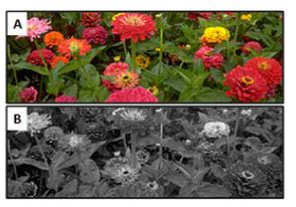
\includegraphics[scale=.5]{grey}\\\\
3) \textbf{Edge Detection}: Edge detection is the technique used to
identify the fine edges in digital images. It identifies the points
in the image at which the brightness of image changes very
sharply. Point at which the image brightness changes are
organized into set of curved line segments known as edges. Edge
detection is mainly an important tool in the field of image
processing for detection of features and feature extraction.
Approaches of edge detectionTwo
main methods of edge detection are search based and zero
crossing based. Search based method detects edges by
computing the edge strength. The zero crossing based method
searches for the zero crossing second-order derivative expression
computed form images in order to find edges.\\\\
4) \textbf{Segmentation}: The aim of segmentation is converting an
image into more meaningful and easy to analyze portions.
Segmentation does the job of partitioning an image into multiple
segments which help to locate the objects and boundaries
(curves, arcs, lines, etc.) in an image. With the help of image
segmentation we can assign a label to each pixel which then
same labels share the certain characteristics. We can characterize
the pixels in a region with respect to the characteristics such as
color, intensity or texture.\\\\
5) \textbf{Feature extraction}: In the fields of machine learning, pattern
recognition and image processing, feature extraction plays an
important role of building derived values which are known to be
the features. These features are intended to be informative, nonredundant,
facilitating the subsequent and generalized steps.
Extracted features should contain relevant data from input data.
This technique plays an important task in our proposed system.
Feature Extraction is the key concept in CBIR. A certain number
of features for each image are extracted, describing its high level
content information. Then, according to the similarity of these
vectors, we can compare two specific images to each other. This
class uses different techniques to extract features related to a
single or the group of images. There are two methods in this
class which extracts the features:
 - extractSingleImage : which extracts the features for a single
image. It is used to extract the features of the input image.\\\\
6) \textbf{Speech Synthesis}: It is the process of artificially producing
the human speech. Systems used for such purpose are called
speech synthesizer which can be a software or hardware product.
Concatenations of several pieces of recorded speech are stored in
database and then synthesized speech is created.
A text -to-speech conversion system is used in our work to
convert the generated text of images into speech output. 
\newpage
\subsection{Synergy between Object Recognition and Image
Segmentation}
\textbf{\small \\Y.Ramadevi, B.Kalyani, T.Sridevi }
\\\\\\
Image segmentation is the foundation of object
recognition and computer vision. In general, image noise
should be eliminated through image preprocessing. And
there is some specifically-given work (such as region
extraction and image marking) to do after the main
operation of image segmentation for the sake of getting
better visual effect. Two major computer vision problems,
image segmentation and object recognition, have been
traditionally dealt with using a strict, bottom-up ordering. \\
Image segmentation is to partition an image into
meaningful regions with respect to a particular
application. The segmentation is based on measurements
taken from the image and might be grey level, colour,
texture, depth or motion. The result of image segmentation
is a set of segments that collectively cover the entire
image.\\
Object recognition is the task of finding a given
object in an image or video sequence. For any object in an
image, there are many 'features' which are interesting
points on the object that can be extracted to provide a
"feature" description of the object. This description
extracted from a training image can then be used to
identify the object when attempting to locate the object in
a test image containing many other objects. \\\\
1)\textbf{Segmentation} Edge-based segmentation partitions an image
based on abrupt changes in intensity near the edges
whereas region-based segmentation partitions an image
into regions that are similar according to a set of
predefined criteria. Region-based segmentation looks for
uniformity within a sub-region, based on a desired
property, e.g. intensity, color, and texture as shown figure
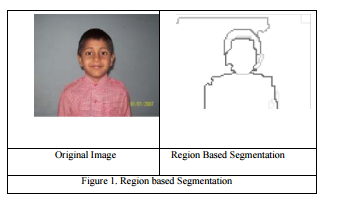
\includegraphics[scale=.5]{1}
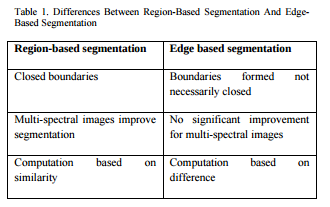
\includegraphics[scale=.5]{2}\\\\
2)\textbf{Active contours} are popular technique for image
segmentation. An advantage of active contours as image
segmentation methods is that they partition an image into
sub-regions with continuous boundaries. There are two
kinds of active contour models according to the force
evolving the contours: edge- and region-based. Edgebased
active contours use an edge detector, usually based
on the image gradient, to find the boundaries of subregions
and to attract the contours to the detected
boundaries. Region-based active contours use the
statistical information of image intensity within each
subset instead of searching geometrical boundaries as
shown in figure. \\
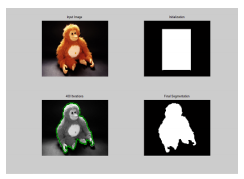
\includegraphics[scale=.5]{3}\\\\
3)\textbf{Image Segmentation} the generative models are used
to decide which part of the image a model should occupy.
Active Appearance Model (AAMs) is used as generative
models and addresses the problem of jointly detecting and
segmenting objects in images. Regarding recognition,
each object hypothesis is validated based on the image
area assigned to the object, as well as the estimated model
parameters, which indicate the familiarity of the object
appearance. On one hand, knowing the area occupied by
an object is needed for the estimation of the model
parameters and, on the other hand, the model synthesis is
used to assign observations to the model. Since neither is
known in advance, we cannot address each problem
separately. We view this problem as an instance of the
broader problem of parameter estimation with missing
data: In our case, the missing data are the assignments of
observations to models. A well-known tool for addressing
such problems is the EM algorithm.\\\\
4)\textbf{Expectation-Maximization} (EM) algorithm
is used for finding maximum likelihood estimates of
parameters in probabilistic models, where the model
depends on unobserved latent variables. In order to find
maximum likelihood estimate we have to find probability
density function and loglikelihood. \\
The EM algorithm is an efficient iterative
procedure to compute the Maximum Likelihood (ML)
estimate in the presence of missing or hidden data. Each
iteration of the EM algorithm consists of two processes:
The E-step, and the M-step. In the expectation, or E-step,
the missing data are estimated given the observed data and
current estimate of the model parameters. This is achieved
using the conditional expectation, explaining the choice of
terminology. In the M-step, the likelihood function is
maximized under the assumption that the missing data are
known. The estimates of the missing data from the E-step
are used in lieu of the actual missing data.
The EM algorithm seeks to find the MLE by
iteratively applying the following two steps:
\begin{itemize}
\item Expectation step: Calculate the expected value of
the log likelihood function, with respect to the conditional
distribution of z given x under the current estimate of the
parameters $\theta (t)$ .
\item Maximization step: Find the parameter which
maximizes this quantity. 
\end{itemize}
5)\textbf{Image segmentation using OTSU}
,OTSU algorithm is based on the point of image
segmentation in the global threshold selection. This
method of its calculation is simple, stable and effective,
has been widely used still image processing toolbox
MATLAB gray image as the threshold value
automatically select a single standard algorithm. The
OTSU method is one of the applied methods of image
segmentation in selecting threshold automatically for its
simple calculation and good adaptation.
In image processing, OTSU’s thresholding
method is used for automatic binarization level decision,
based on the shape of the histogram. The algorithm
assumes that the image is composed of two basic classes:
Foreground and Background. It then computes an optimal
threshold value that minimizes the weighted within class
variances of these two classes. It is mathematically proven
that minimizing the within class variance is same as
maximizing the between class variance.
The thresholding techniques are categorized into
six groups as:\\
\begin{enumerate}
\item Histogram shape-based methods, where
histogram of image is viewed as a mixture of two
Gaussian distributions associated to object and
background classes, such as convex hull
\item Clustering-based methods, where gray-level
pixels are clustered in two classes as either
background and foreground objects or alternately
modeled as mixture of two Gaussians, such as
iterative thresholding, clustering thresholding,
minimum error thresholding and fuzzy clustering
thresholding.
\item Entropy-based methods use difference in entropy
between foreground and background regions,
such as, entropy thresholding.
\item Object attribute-based methods; find measure of
similarity (fuzzy shape similarity, edge
coincidence, etc) between gray-level and
binarized images, such as edge field matching
thresholding and topological stable-state
thresholding.
\item Spatial methods, use higher-order probability
distribution and/or correlation between pixels,
such as higher order entropy thresholding.
\item Local methods, calculate threshold value at each
pixel based on local image characteristics, such
as local contrast method and surface-fitting
threshold.
\item The major problem with thresholding is that we
consider only the intensity, not any relationships between
the pixels. There is no guarantee that the pixes
\end{enumerate}
6)\textbf{Image segmentation} using Genetic Algorithm
Genetic Algorithms (GAs) can be seen as a
software tool that tries to find structure in data that might
seem random, or to make a seemingly unsolvable problem
more or less 'solvable'. GAs can be applied to domains
about which there is insufficient knowledge or the size
and/or complexity is too high for analytic solution.
 Basically, a genetic algorithm consists
of three major operations: selection, crossover, and
mutation. The selection evaluates each individual and
keeps only the fittest ones in the population. In addition to
those fittest individuals, some less fit ones could be
selected according to a small probability. The others are
removed from the current population. The crossover
recombines two individuals to have new ones which might
be better. The mutation operator induces changes in a
small number of chromosomes units. Its purpose is to
maintain the population diversified enough during the
optimization process



\bibliographystyle{apalike}

\bibliography{sample}

%----------------------------------------------------------------------------------------


\end{document}